\section{Repaso}

La intención de las siguientes preguntas es repasar y recordar algunos conceptos básicos que debe tener en cuenta para desarrollar esta tarea e iniciar el curso de cálculo integral.

\begin{itemize}
    \item \textit{Pregunta 1} ¿Qué es una función real, el dominio, el rango y la gráfica de una función real?
    \item \textit{Pregunta 2} ¿Cuál es la definición de valor absoluto?
    \item \textit{Pregunta 3} ¿Qué relación existe entre el concepto de límite de una sucesión o una función con el concepto de valor absoluto?
    \item \textit{Pregunta 4} ¿Qué significa que exista y calcular, el límite de una función real en un punto de su dominio?
    \item \textit{Pregunta 5} ¿Qué es la derivada de una función real en un punto de su dominio? Explique en sus palabras el significado de tasa de cambio instantáneo, qué es la recta tangente a la gráfica de una función en un punto de su dominio, si todas las funciones reales son diferenciables y si el concepto de derivada es global o local en el dominio.
    \item \textit{Pregunta 6} ¿Cuál es la relación entre el concepto de límite y el de derivada?
    \item \textit{Pregunta 7} Resolver e interpretar (es decir, traducir su significado) las siguientes ecuaciones o desigualdades (sugerencia: repasar propiedades del valor absoluto):
\end{itemize}


%%Primera inecuacion
\hspace*{1cm}$|2x-1|-|x+5|=3$

\begin{align*}
    |2x-1| &=
    \begin{cases}
        2x-1, & x \geq \frac{1}{2}, \\
        -(2x-1), & x < \frac{1}{2},
    \end{cases} \\
    |x+5| &=
    \begin{cases}
        x+5, & x \geq -5, \\
        -(x+5), & x < -5.
    \end{cases}
\end{align*}

\subsection*{Gráfica de los intervalos}

\begin{center}
    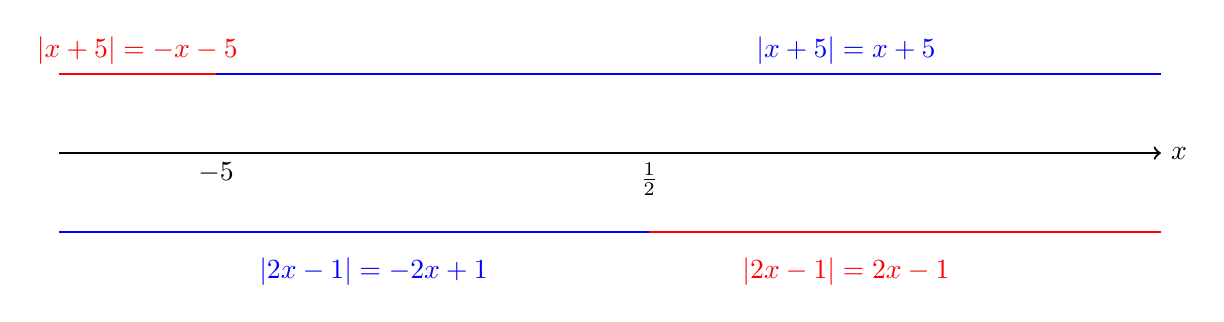
\begin{tikzpicture}[scale=1]
        % Eje horizontal
        \draw[->, thick] (-7,0) -- (7,0) node[right] {$x$};
        
        % Marcas en el eje x
        \draw (-5,0) node[below] {$-5$};
        \draw (0.5,0) node[below] {$\frac{1}{2}$};
        
        % Intervalos
        \draw[red, thick] (-7,1) -- (-5,1);
        \draw[blue, thick] (-5,1) -- (7,1);
        \draw[blue, thick] (-7,-1) -- (0.5,-1);
        \draw[red, thick] (0.5,-1) -- (7,-1);
        
        % Etiquetas mejor ubicadas
        \node[red, above] at (-6,1) {$|x+5|=-x-5$};
        \node[blue, above] at (3,1) {$|x+5|=x+5$};
        \node[blue, below] at (-3,-1.2) {$|2x-1|=-2x+1$};
        \node[red, below] at (3,-1.2) {$|2x-1|=2x-1$};
    \end{tikzpicture}
\end{center}

\subsection*{Resolución por casos:}

\textbf{Caso 1}: \(x < -5\)
\begin{align*}
    -(2x-1) - \big[-(x+5)\big] &= 3,\\[1mm]
    -2x+1 + x+5 &= 3,\\[1mm]
    -x+6 &= 3,\\[1mm]
    -x &= -3,\\[1mm]
    x &= 3.
\end{align*}
\textbf{Conclusión}: \(3 \notin (-\infty,-5)\) \quad (\textbf{No es solución})

\textbf{Caso 2}: \(-5 \leq x < \frac{1}{2}\)
\begin{align*}
    -(2x-1) - (x+5) &= 3,\\[1mm]
    -2x+1 - x-5 &= 3,\\[1mm]
    -3x-4 &= 3,\\[1mm]
    -3x &= 7,\\[1mm]
    x &= -\frac{7}{3} \approx -2.33.
\end{align*}
\textbf{Conclusión}: \(-\frac{7}{3} \in \left[-5, \frac{1}{2}\right)\) \quad (\textbf{Solución válida})

\textbf{Caso 3}: \(x \geq \frac{1}{2}\)

\begin{align*}
    (2x-1) - (x+5) &= 3,\\[1mm]
    2x-1 - x-5 &= 3,\\[1mm]
    x-6 &= 3,\\[1mm]
    x &= 9.
\end{align*}

\textbf{Conclusión}: \(9 \in \left[\frac{1}{2}, \infty\right)\) \quad (\textbf{Solución válida})\\
\subsection*{Solución general}
\begin{equation*}
    x = \frac{-7}{3}, 9
\end{equation*}




%%Segunda inecuacion
\hspace*{1cm}$|x-1|-|x-3|\geq 5$
\begin{align*}
    |x-1| &= \begin{cases}
        x-1, & x \geq 1, \\
        -(x-1), & x < 1.
    \end{cases} \\
    |x-3| &= \begin{cases}
        x-3, & x \geq 3, \\
        -(x-3), & x < 3.
    \end{cases}
\end{align*}

\subsection*{Gr\'afica de los intervalos}

\begin{center}
    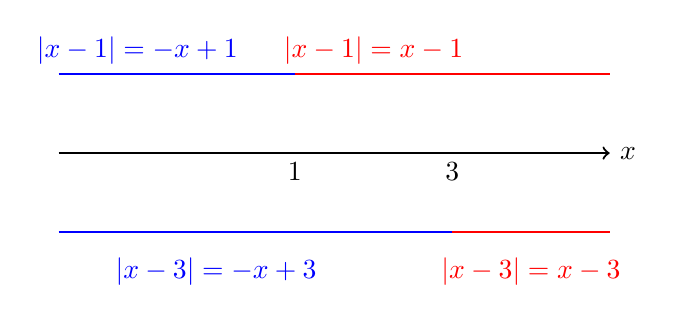
\begin{tikzpicture}[scale=1]
        % Eje horizontal
        \draw[->, thick] (-2,0) -- (5,0) node[right] {$x$};
        
        % Marcas en el eje x
        \draw (1,0) node[below] {$1$};
        \draw (3,0) node[below] {$3$};
        
        % Intervalos
        \draw[blue, thick] (-2,1) -- (1,1);
        \draw[red, thick] (1,1) -- (5,1);
        \draw[blue, thick] (-2,-1) -- (3,-1);
        \draw[red, thick] (3,-1) -- (5,-1);
        
        % Etiquetas mejor ubicadas
        \node[blue, above] at (-1,1) {$|x-1|=-x+1$};
        \node[red, above] at (2,1) {$|x-1|=x-1$};
        \node[blue, below] at (0,-1.2) {$|x-3|=-x+3$};
        \node[red, below] at (4,-1.2) {$|x-3|=x-3$};
    \end{tikzpicture}
    \end{center}
    

\subsection*{Resoluci\'on por casos}

\textbf{Caso 1}: $x < 1$
\begin{align*}
    (-x+1) - (-x+3) &\geq 5,\\
    -x+1 + x -3 &\geq 5,\\
    -2 &\geq 5.
\end{align*}
\textbf{Conclusi\'on}: Falso \quad (\textbf{No hay soluci\'on})

\textbf{Caso 2}: $1 \leq x < 3$
\begin{align*}
    (-x+3) - (x-1) &\geq 5,\\
    -x+3 - x +1 &\geq 5,\\
    -2x +4 &\geq 5,\\
    -2x &\geq 1,\\
    x &\leq -\frac{1}{2}.
\end{align*}
\textbf{Conclusi\'on}: $-\frac{1}{2} \notin [1,3)$ \quad (\textbf{No hay soluci\'on})

\textbf{Caso 3}: $x \geq 3$
\begin{align*}
    (x-3) - (x-1) &\geq 5,\\
    x-3 - x +1 &\geq 5,\\
    -2 &\geq 5.
\end{align*}
\textbf{Conclusi\'on}: Falso \quad (\textbf{No hay soluci\'on})

\subsection*{Soluci\'on general}

\begin{equation*}
    \text{No hay soluciones reales.}
\end{equation*}




%%Tercera inecuacion
\hspace*{1cm}\textbf{$|x^2-1|\leq \frac{1}{2}$}

\[
-\frac{1}{2} \leq x^2 - 1 \leq \frac{1}{2}
\]

\textbf{Primera desigualdad}
\[
-\frac{1}{2} \leq x^2 - 1
\]
\[
-\frac{1}{2} + 1 \leq x^2
\]
\[
\frac{1}{2} \leq x^2
\]
\[
|x| \geq \sqrt{\frac{1}{2}}
\]
\[
x \leq -\sqrt{\frac{1}{2}} \quad \text{ó} \quad x \geq \sqrt{\frac{1}{2}}
\]

\textbf{Segunda desigualdad}

\[
x^2 - 1 \leq \frac{1}{2}
\]
\[
x^2 \leq \frac{1}{2} + 1
\]
\[
x^2 \leq \frac{3}{2}
\]
\[
|x| \leq \sqrt{\frac{3}{2}}
\]
\[
-\sqrt{\frac{3}{2}} \leq x \leq \sqrt{\frac{3}{2}}
\]

\begin{center}
    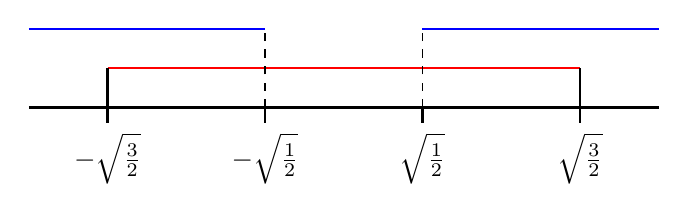
\begin{tikzpicture}
        % Eje
        \draw[thick] (-4,0) -- (4,0);
        
        % Puntos en la recta con etiquetas corregidas
        \draw[thick] (-3,0) --++ (0,-0.2);
        \node[below] at (-3,-0.2) {$-\sqrt{\frac{3}{2}}$};
    
        \draw[thick] (-1,0) --++ (0,-0.2);
        \node[below] at (-1,-0.2) {$-\sqrt{\frac{1}{2}}$};
    
        \draw[thick] (1,0) --++ (0,-0.2);
        \node[below] at (1,-0.2) {$\sqrt{\frac{1}{2}}$};
    
        \draw[thick] (3,0) --++ (0,-0.2);
        \node[below] at (3,-0.2) {$\sqrt{\frac{3}{2}}$};
    
        % Intervalo cerrado en rojo (-sqrt(3/2), sqrt(3/2))
        \draw[thick, red] (-3,0.5) -- (3,0.5);
        \draw[thick] (-3,0) -- (-3,0.5);
        \draw[thick] (3,0) -- (3,0.5);
        
        % Intervalos abiertos en azul (-∞, -sqrt(1/2)) y (sqrt(1/2), ∞)
        \draw[thick, blue] (-4,1) -- (-1,1);
        \draw[thick, blue] (1,1) -- (4,1);
        \draw[dashed] (-1,0) -- (-1,1);
        \draw[dashed] (1,0) -- (1,1);
        
    \end{tikzpicture}
\end{center}


\textbf{Solución:} 
\begin{equation*}
    x \in \left[-\sqrt{\frac{3}{2}}, -\sqrt{\frac{1}{2}}\right] \cup \left[\sqrt{\frac{1}{2}}, \sqrt{\frac{3}{2}}\right].
\end{equation*}


\textit{Pregunta 8. Evalúe los siguientes límites:}

\begin{enumerate}
    \item $ \lim\limits_{x \to 2} \frac{x^2 - 4}{x - 2} $
    
    \textbf{Caso: Diferencia de Cuadrados}
    \[ \lim\limits_{x \to 2} \frac{(x+2)(x-2)}{x-2} = \lim\limits_{x \to 2} x+2 = 4 \]
    
    \item $ \lim\limits_{x \to 0} \frac{\sin x}{x} $
    
    \textbf{Regla de L'Hôpital}
    \[ \lim\limits_{x \to a} \frac{f(x)}{g(x)} = \lim\limits_{x \to a} \frac{f'(x)}{g'(x)} \]
    Para los casos $ \frac{0}{0} $ o $ \frac{\infty}{\infty} $:
    \[ \lim\limits_{x \to 0} \frac{\cos x}{1} = \frac{1}{1} = 1 \]
    
    \item $ \lim\limits_{x \to \infty} \frac{3x^2 + 5}{2x^2 - 7} $
    
    \textbf{Se divide todo por el mayor exponente}
    \[ \lim\limits_{x \to \infty} \frac{K}{x^n} = 0 \]
    
    \[ \lim\limits_{x \to \infty} \frac{\frac{3x^2}{x^2} + \frac{5}{x^2}}{\frac{2x^2}{x^2} - \frac{7}{x^2}} = \frac{3 + 0}{2 - 0} = \frac{3}{2} = 1.5 \]
    
\end{enumerate}